\documentclass{article}
\usepackage[utf8]{inputenc}
\usepackage{amsmath}
\usepackage{amssymb}
\usepackage{graphicx}
%\usepackage[margin=1.35in]{geometry}


\author{Henry Yang : 19940503-1056}
\title{Wizard Of Wor \\\large a report for the course \\TDA572 (Game Engine Architectures)}
\date{Mars 2018}

\begin{document}
  \maketitle
  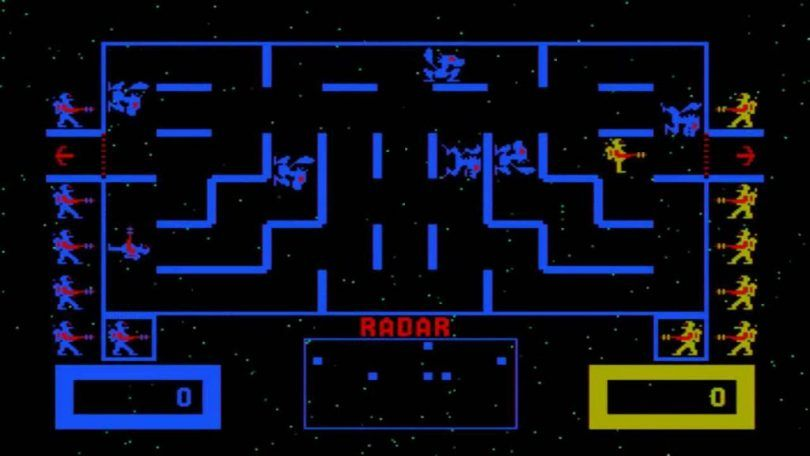
\includegraphics[scale=0.4]{assets/lateximg/WizardOfWor}\\
  Image Source: \texttt{https://www.moregameslike.com/}
  \section{Introduction}

  This report is a report for the development of a clone of the 80's Arcade game \textbf{Wizard Of Wor}. The game said game, which this project is a clone of is an arcade game developed by Midway. This report will start by introducing the reader to the original Game, identifying the gameplay mechanics of the game, and other important key-features of this game.

  We will than go on and identifying the possible problems to be solved when creating a game like Wizard Of Wor and the solutions for these. In the same section, we will also discuss the viability of implementing all the possible features of this game. Since the there are many features in the said game, some of the features that are present in the original game will be omitted. This will be discussed here.

  The report will than go on to discuss the design the development process of the game, as well as challenges that surfaced during development. Additionally, this section will discuss the decision made regard the design and implementation of the features of the game.

  In the next section, the report will showcase, and discuss the results of the project. What could be done differently, future plans, and other discussions related to the project.

  \subsection{Project structure and Libraries}
  The whole project is written in the language C++, which is a common language found within the area of Game development. The language itself is notable for it's low-level nature and being very close to hardware level, thus it is also by implication very high performing programming language.

  Addtionally, the project will use SDL, which is a library that is very commonly used within game development. According to Wikipedia, SDL is a library that provides an hardware abstraction layer for computer multimedia hardware components. In other words, the library is similar to OpenGL, but provides more functionallities than OpenGL, which is a library used for computer graphics. Examples of titles that are developed using SDL are \textbf{Brütal Legend}, \textbf{Memoria}, and \textbf{Robin Hood}.

  \section{Background and Specification}
  This section will break down the original game, and from it identify the key-features and specifications for it, thus also for this project as a whole.

  \begin{figure}
    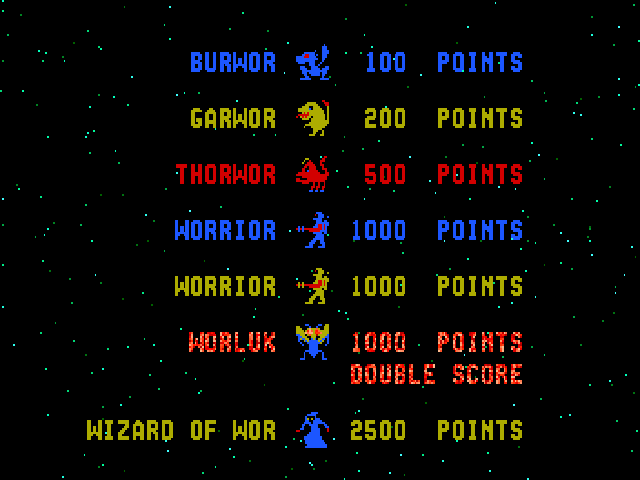
\includegraphics[scale=0.7]{assets/lateximg/Monstertable}
    \caption{The Table of the monsters in the game, including the both players (the Worriors). Source: \texttt{https://extralives.files.wordpress.com}}
    \label{monstertable}
  \end{figure}

  \subsection{The Original Game}

  The original game is playable by up to two people. The players, also known as \textbf{Worriors} in the game, are running around in a two dimensional maze with a lot of Monsters. The objective is to gather as much score as possible. Score points is acquired by killing the monsters in the Maze. When a maze is cleared, they move on two the next level, which is another maze filled with monsters. The end score is the collective points collected from the process of killing monster and clearing as many levels as possible. Each maze has it's own difficulties in the form of how design, and amount of monsters.

  In the case that two players are playing the game. The players can also gather points by killing each other.

  The players loses lives if they are killed by the monsters. From the beginning, each player starts with 3 lives. Monsters can kill the player by firing on them and by walking into the player. Hence, the player will die if he/she collides with a monster.

  There are 5 different typse of monsters in this game, each worth different amounts of points and have different attributes to them. These can be found in the picture figure \ref{monstertable}.

  A more detailed explanation of the monsters:
  \begin{itemize}
    \item \textbf{The Burwor}: The easiest monster to kill, no special features, and moves a little bit slower than the players.
    \item \textbf{The Garwor}: A monster that is similar to the Burwor, but can become invisible.
    \item \textbf{The Thorwor}: This monster is faster than the Burwor and the Garwor. It is also capable of going invisible.
    \item \textbf{The Worluk}: This monster will not attack the players, instead, it will try to escape the maze. The player will still pass the level if this monster escaped, but killing the monster will give the player double points in the next level. Note that this monster moves very fast
    \item \textbf{The Wizard of Wor}: This monster is kind of main boss, though it is still killed with one shot, it moves faster than all the other monsters except for the Worluk. It is also capable of teleportation. Not that the game is named after this monster.
  \end{itemize}

  In addition, as mentioned in the introduction, the Worriors, i.e. the player can also kill eachother, with a profit of 1000 points each kill, the tradeoff in doing so is that the killing of the other monster will be harder. However, note that killing the other player awards more points than at least 3 of the monsters. Thus a very interesting situation of two players \textbf{Prisoners Dilemma} arises in this game(See appendix).

  Other interesting features of this game is the use of voice synthetisation in form of tauntings performed by the Wizard of Wor himself.

  \subsection{Key features and project specifications}
  From the previous subsection following key features can be found:
  \begin{itemize}
    \item Two Players Control.
    \item The Maze - Each level is a different maze. This also includes the movemente in the maze.
    \item AI - Each monster moves on it's own according to an AI, making this game a multiagent system with many different agents. Note that there are 5 unique types of monsters in this game, thus around 5 different kind of AI's in the game.
    \item Collision detection with the projectiles, and the monsters.
    \item Sound- and voice synthetisation for the sound samples and the tauntings by the wizard.
    \item Other aesthetics such as animations, and different sprites.
  \end{itemize}
  This project will try to implement as many key-features as possible, but focuses mainly on the first four. This is beacuse the last 2 are mainly for aesthetics of the game, thus not a key mechanics for the game itself. These will be implemented if time allows it to.

  \subsection{Problems present}
  There are different kind of problems to be solved, if one ought to make a clone of Wizard Of Wor. This subsection will take the problems related to the key-features as identified in the last subsection.

  First of, the whole two players game notion is a problem by itself. Not only does it relate to the main mechanics of the game. It also relates a lot to the user experience from the players playing this game. Finding a good set of controlls can be identified as a challenge in the making of this game.

  Moving on to the maze, One of the main problems that the maze introduces to the game is the movement, and bounding each entity inside the maze. There are various ways of representing the maze internally in the game, thus finding the optimal model for the maze is a problem by itself. This problem also relates to the player controll stated in the last paragraph. It also influences the modelling of the AI for the monsters.

  As already stated above, collision detection is needed in this game. There are two kinds of collision to detect. The Players and monsters against a projectile, and the collision monster against player.

  The AI is probably one of the most complex of these problems, This can be broken down into two types of problems: Path finding and Heuristics. There are many algorithms for path searching, including depth first, and breadth first search. There are greedy approaches and algorithms related to dynamic programming. Heuristics problems are related to the path findings, since using good heuristics can greatly influence the performance in time complexity of the path searching algorithm. Heuristics are also good for differentiate each of the unique AI controlled entities behaviour pattern. In this game, due to the existence of reload time, a Heuristics for when to shoot a projectile is important.

  \subsection{Extension}
  IN addition to the above mentioned features. A decision was made to extend the functionallities of AI to also make it possible for a single-player-AI co-up mode. This is so that the game might be enjoyable even though there is only one player. One of the main challenges with this can once again be referred to the occurences of the prisoners dilemma from the core gameplay for two players. This will be discussed later.

  \section{Implementation}
  This section will give a short description of the development process outlining the design, and modelling choices made, as well as the challenges that came up related to the development of this game. In the beginning of the project, we were given a set of C++ code as a starting point.

  In this library Basic implementation of a gameloop, a basic set of classes representing the game objects, and each objects components, a basic implementation of a player, and a set of classes that provides functionalities like rendering of sprites and basic IO handling. In addition, a basic implementation of collision detection, and collision handling are implemented.
  Other useful code that were provided are basic implementation of an object pool among other useful utilities.

  \subsection{Class Hierarchy and code structure}
  C++ as a language provides many useful features that is not seen in it's predecessor C. This includes Object orientation. This projects makes use of this in different ways.

  In this project, the main class-Hierarchy are focused around the \texttt{Component} and \texttt{GameObject} classes. Every thing in the game can be viewed as a GameObject instance. This includes the Tiles in the maze, and every moving entity. Every GameObject have at least one component that handles the rendering of the said GameObject. A moving GameObject uses at least one component that are used to handle the movement, and behaviour of the Moving Game Object.

  It doesn't take long to realise that this game uses a MVC like software architecture design. With the components acting as a part of the Controller and view handling updating and reading the GameObjects.

  During the project additionall subclasses to the two base classes was introduced. This includes a \texttt{MovingGameObject} class that handles the moving directions. Another subclass to \texttt{GameObject} is the \texttt{Collidable} class that are used for collision handling, this is so that the visitor pattern could be used for collision handling. In this project, the \texttt{Collidable} class is a subclass to \texttt{MovingGameObject}.

  The ideal design decision would be to have these as two different classes. However, that introduces an inheritance problems one a GameObject is both Moving and Collidable. This is the infamous Diamond structure, which is a not really a desired inheritance structure if their common superclass have data fields. Since most of the Moving entites are also collidable , with Projectiles being an exception since they can only "collide with" other entities but not collided on.
  Thus the decision to make \texttt{Collidable} into a subclass for \texttt{MovingGameObject} was made. Appart from that, almost every entity in the game is represented by a subclass.

  One of the most significant subclass to the \texttt{Component} is the \texttt{AIComponent} class which serves as a basic class for AI behaviour. An notable subclass to that is the \texttt{AstarAIComponent} class, which is the base class for an AI using the $A^*$ path searching algorithm. The AIComponent also holds an instance of the \texttt{Heuristics} to utilise the Strategy pattern for computing different heuristics.

  \subsection{Two Players Controll}
  This was more of a design problem rather than an implementation problems. Since the provided classes already handles the oneplayer-case movement. Minor modifications to the provided code was made to handle the controll of a second player. The first player (WorriorGold) uses the popular "WASD" controlls and fires with "C".

  While not using WASD, the second human player uses "IJKL" for movement, and "." for firing. This design decision was made so that the hand pattern will remains the same since the controlls are only shifted to the other half of the keyboard.

  An issue might occure with the players body alignment from these controlls, since both controlls are biased towards right-handed controlls. User testing indicates that this is not really a significant problem.

  \subsection{The Map}
  The modelling and implementation of the Map is very important as described in the previous section.

  The initial implementation of the map is a two dimensional grid of tiles that represent what kind of walls there is to render at a coordinate in the tile grid. Each tile has a dimension of $32\times32$ in the pixel grid space of the actuall model. This model closely represents how the maze is represented graphically.

  To get the current tile each entity was on, the players coordinates are divided by 32 and than moved by the map offset to the screen. Rounding this number will get the Tile that mostpart of the entity is standing in. Though the model sounds simple, it makes the wall collision very verbose, and very logic heavy driven by boolean statements. A bug that was present in the game while using this model was that the entities could "Walk through wall" since the Game though that it was standing on a tile where there is no wall in a said direction.

  Due to the above mentioned bug, and other problems, mostly related to the realization of an AI, A complete overhaul of the map model was made. A binary matrix $M$ where each $32\times32$ chunk submatrix represent a specific tile was made. If value 1 is found on $M_{xy}$, than there was a probably a wall in that chunk of pixels. This model greatly simplified the Wall detection during movement.

  A design decision made was to keep the tile map grid, since it greatly simplifies the rendering of the maze, as well as providing some helpful utilities to handle some smart player movement controll to make some controlls easier.

  The map is also stored in text format before the game actually starts and being loaded inside the game. Currently, the standard map is stored within the sourc ecode.

  \subsection{AI}
  As mentioned in a previous subsection, the AI greatly relays on the Strategy pattern for heuristics. At the point of writing this report, only one piece of AI was implemented that uses the $A^*$ Path finding algorithm. Different kind of were considered upon. At the time of writing this report, none was actually realised. Note that this might not be the case in the final results that was handed in.

  The original plan was to implement a firing heuristics that tells the AI to shot if able when the target is in the vicinity of about three tiles. More of this is discussed in the Future work section.

  \section{Results and Discussion}
  \begin{figure}
    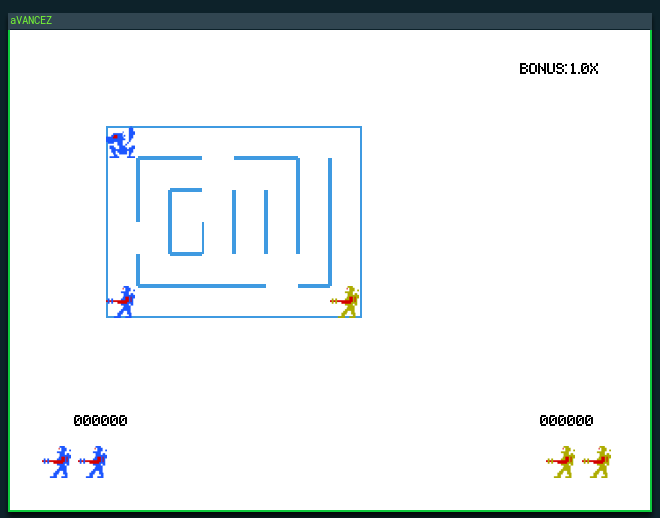
\includegraphics[scale=0.5]{assets/lateximg/InGameScreenshot}
    \caption{The Final results of the development before deadline}
    \label{game}
  \end{figure}

  The final results of the project are showcased in figure \ref{game}. Among the keyfeatures, the player controlls, collision detection, as well as the implementation of a Maze. Although, classes and a framework is present in a code, as well as an implementation of the $A^*$ algorithm. At the time of writing, none of this was actually realised thus the last AI-key feature cannot be considered complete. Note that this is at the time of writing this report.

  The current game has no monsters outside of a simple burwor to showcase collision handling and the scoring. As well as a small maze to showcase the movement. Also, currently the game can be played by two players with the controlls that are described in the last section.

  Mainly due to the AI-parts, and the aesthetics not fully implemented as of yet. The Project cannot be considered complete as of writing this report.

  \subsection{Challenges and Setbacks}
  There were many challenges faced during the project development. Many of those are related to C++ and the inexperience with it. Due to the nature of C++ as a compiled language and the massive codebase, testing new pieces of written code like classes and functions are not easlily performed without rewriting the \texttt{main.cpp} file. This, accommodated with the side-effects oriented logic base of the code made it incredibly hard to debug certain behaviours.

  One such issues are segmentation faults, which are results from reading on non valid memory addresses among other causes. Another examples of issues arises forinstance when reading outside array boundaries, sometimes, this doesn't give a segmentation faults, but can result in strange behaviours that is even harder to debug than segmentation faults.

  The overall complexity of the game and it's various systems can also be considered a challenge. Especially for a single man team like this one. The fact that the team member himself isn't that experienced with either C++ or Game development in general, the project took much longer time than expected. For example, finding the optimal representation of a maze took much longer time, and a complete overhaul to finally be usable.

  Complexity is one thing, but one of the main reasons for this uncompleted project is due to bad time-planning as well as underestimation of the complexity of the game itself. The bad time-planning is be described as a combination of underestimating the problem complexity, inexperience with the given tools and languages. This in term also resulted in dedication to other projects and courses. The bad time planning it self is also a result of inexperience within game development in general, as well as bad motivation versus ambition.

  \subsection{Future Work}
  A thing that could be done in the future is to finish the game and make it a closer clone to the original with the addition of single AI-Player Co-up mode. This involves implementing, and realising more Maps and implement the animations and sound effects. This is already doable by creating subclasses to the \texttt{RenderComponent} class that came with the initial code base.

  Another intersting thing would be to utilising and implementing heuristics of stochastic nature,and more search algorithms for path finding. One such algorithm could be monte-carlo tree-search for path finding for instance. Finding a good heuristics for shooting would be one of the things that would be an interesting exploration area for the future since there are many ways this could be done.

  The most interesting part is to implement a more sophisticated stochastic heuristics for the Player2-AI. Forinstance having a trained Neural Network, that could evaluate the overal profit of taking a certain turn. This is especially interesting due to the prisoners dilemma situation. One can explore weather the AI would for instance evaluate the profit vs tradeoff for going after the other player, since according to the basic game theory, the most profitable decision in the prisoners dilemma for a single player would be to betray it's partner. Game theory also tells that the most profitable situation for both players though are to cooperate.

  These among other stuff are interesting things worth experiment with and exploring when developing the player2 AI.

  \section{Conclusion and Final Verdicts}

  To sum up the project, eventhough the game itself was never finished, larger portions of the key-features that was planned for this project was implemented with the AI not really realised in some way as of writing this report. This is largely due to inexperience, bad planning and underestion of the problem complexity.

  Since this is a course in Game Engine Architecture. Being able to learn from the standard problems and the challenges might be a soughtful experince and knowledge. Especially for this team of one student that is inexperienced in the area of game development, and interactive simulations.

  With this in mind, a lot can be learned from this project, esepcially in the time distribution department. But also regarding game engines and game development as a whole. The team memebers would be better geared in the future when facing the problems that took form during the course of the project. Learning to better estimating problem complexity within game development, and time planning are also valuable experience that the team memebers would keep and make use of in the future.

\newpage
  \section{Appendix}
  \subsection{Prisoners Dilemma}

  In the area of Game Theory, the prisoners dilemma is a two players game that can be formulated as following:

  Two people have commited a crime and are in for interogation, they are also facing a sentence of one year in prison. The interogator presents the two parties with a choice to tell on he's or her's partner for 0 years in prison. The partner in crime will be facing a sentence of 5 years. But if both parties tell on each other, they both will face a sentence on 3 years.

  Given these choices of possible outcome. One can quickly infer that the better move in one round of the game for an individual player is to back talk on your partner and betray them. However note that, in if neither betray each other, both faces a collective minimal punishment.

  This is interesting for Wizard Of Wor, since both players are faced with either shooting the monsters in the maze, or shoot the other player for more points. Note that though, betraying eachother has a consequence in Wizard of Wor, the players will have a harder time killing the monsters if they are busy killing each other, and if one of them has depleted their lives.
\end{document}